\documentclass[12pt]{jsarticle}

\setcounter{secnumdepth}{3}
\usepackage[dvipdfmx]{graphicx}
\usepackage{amsmath}
\usepackage{subfigure}

\begin{document}

\section{目的}
 ここでは,熱交換器や強制貫流ボイラのような,熱伝導プロセスの一つである加熱プロセス系を制御対象として,最短時間制御により温度を制御する方法を学ぶ.一般に熱伝導系は,長大ばねの振動や建造物などにおける弾性振動と同様に,時間の他に空間を表す独立変数が必要な分布定数系として取り扱われる.しかし,本実験ではモデル化や制御系構成の簡単化のために対象を集中定数系として取り扱い,熱伝導系のある一点の温度に注目した最短時間制御系を構築する.
\section{実験装置の概要}
 まず,実験装置は図\ref{FigB1}に示されるように上端がヒータによって加熱される構造であり,また,下端に放熱板が取り付けられている銅棒(加熱プロセス),温度測定用の熱電対を用いた測定システム,計算機および変圧器から構成される(図\ref{FigB2}).ヒータに供給される電力は変圧器によって調整可能であり,計算機によって測定温度の記録を行う.\\
 次に加熱プロセスの詳細を図\ref{FigB3}に示す.加熱プロセスは銅棒の表面から熱が拡散するのを抑えるため,保温用の綿が巻き付けられている.銅棒は上端から加熱され,放熱板につながる下端から冷却される.銅棒の各点の温度はシース型熱電対によって測定され,A/D変換器を経て計算機に記録される.
\section{原理}
\subsection{制御対象の伝達関数}
 x[m]をヒータからの距離,t[s]を時間,$\theta(x,t)$[K]をその時の温度とする.初期条件$\theta_x(x,0)=0$(温度勾配が0)でステップ状の入力$Q_0(t)=Q_0$[J]が印加された場合,この系は次式で表現できることが知られている.
\begin{equation}
  \label{B3-1}
  \theta(x,t) = \sum_{n=1}^{\infty}\frac{2}{\pi+2b_n}\frac{Q_0^{\prime}\sin(a_nx)}{xa_n^3}\cos{a_nx(1-e^{-a_n^2t})}
\end{equation}
ただし,$a_n$は$\tan(a_n\pi) = \frac{\alpha^{\prime}}{a_n}$の解であり,また,
\begin{displaymath}
  \alpha^{\prime} = \frac{\alpha L}{\pi}, b_n = \frac{\sin(2\pi a_n)}{4a_n}, Q_0^{\prime} = \frac{L^2Q_0}{\pi^2A_mK}
\end{displaymath}
である.ここで$\alpha$は境界条件を表す定数,$A_m$[$m^2$]は加熱棒の断面積,$L$[m]は加熱棒の長さ,また$K$[J/Kms]は加熱棒の熱伝導率である.式(\ref{B3-1})は位置$x$と時間$t$の関数となるが,ここではある一点$x_0$,すなわち熱電対を取り付けた点に着目した集中定数系とみなし,その近似伝達関数を求める.なお,式(\ref{B3-1})は厳密には無限級数の形で表されるが,三次以上の後は十分小さいので二次系とみなせる.さらに,本実験では簡単のため,近似伝達関数を(一次遅れ) + (むだ時間) の形で導出する.このような近似を行っても実用上はほとんど問題,制御系の設計など後の処理が簡便になるので,実システムの設計や運用にもよく用いられる.
さて以下では,求めるプラントの伝達関数$G_p$を次式で与え,同定実験により未知パラメータ$K_p$,$T_p$,$L_p$を決定することを考える.
\begin{equation}
  \label{B3-2}
  G_p = \frac{K_p}{1+T_ps}e^{-L_ps}
\end{equation}

%\begin{figure}[htb]
%  \begin{center}
%    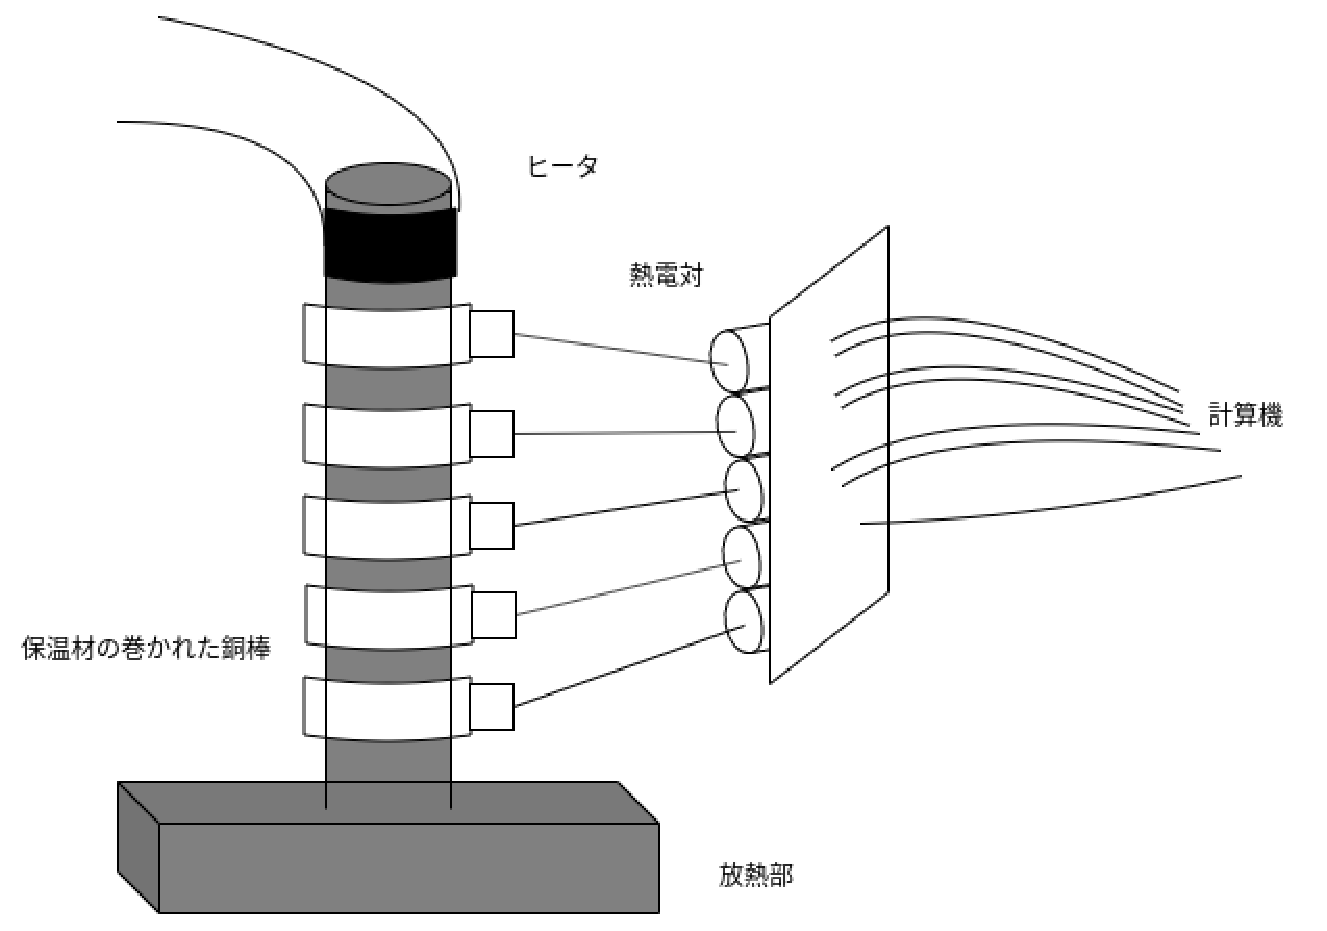
\includegraphics[clip,width=4.0cm]{../Img/FigB1.eps}
%    \label{FigB1}
%    \caption{実験装置の概観}
%  \end{center}
%\end{figure}
%
%\begin{figure}[htb]
%  \begin{center}
%    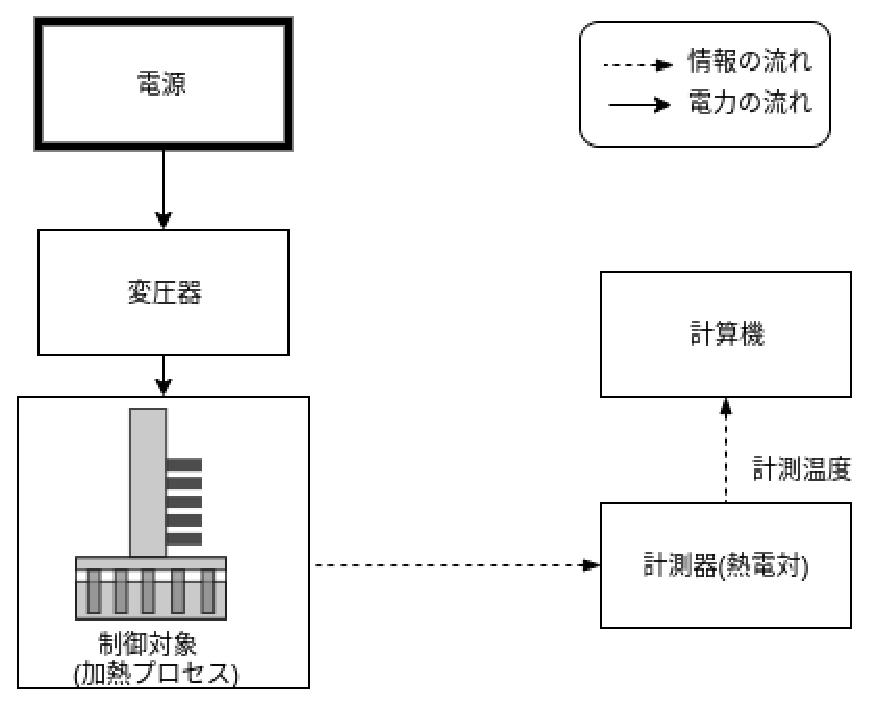
\includegraphics[clip,width=4.0cm]{../Img/FigB2.eps}
%    \caption{実験装置の概要}
%    \label{FigB2}
%  \end{center}
%\end{figure}

\begin{figure}[htbp]
 \begin{minipage}{0.5\hsize}
  \begin{center}
    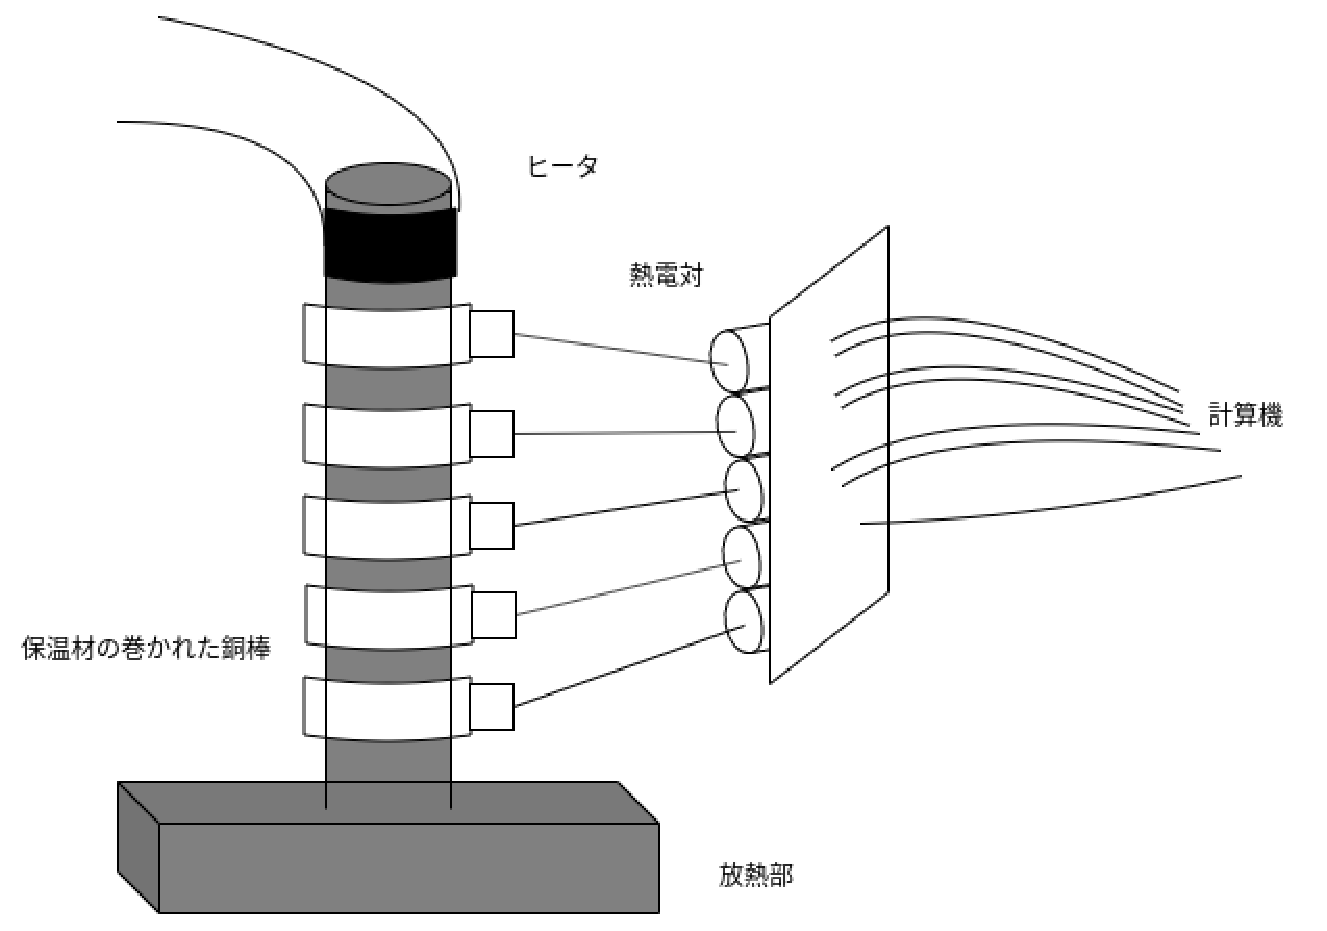
\includegraphics[clip,width=4.0cm]{../Img/FigB1.eps}
  \end{center}
  \caption{実験装置の概観}
  \label{FigB1}
 \end{minipage}
 \begin{minipage}{0.5\hsize}
  \begin{center}
   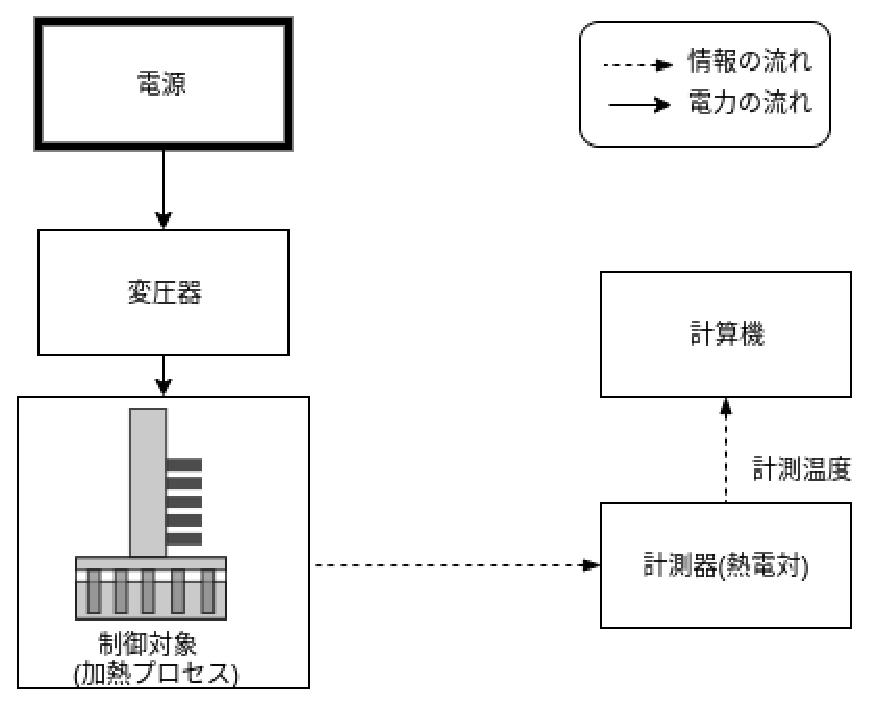
\includegraphics[clip,width=4.0cm]{../Img/FigB2.eps}
  \end{center}
  \caption{実験装置の概要}
  \label{FigB2}
 \end{minipage}
\end{figure}
%\begin{figure}
%  \begin{center}
%  \subfigure[実験装置の概観]{
%    %\begin{pspicture}...\end{pspicture}
%    %\input{graphics.tex}
%    %\resizebox{0.49\textwidth}{!}{\input{hogehoge.tex}}
%    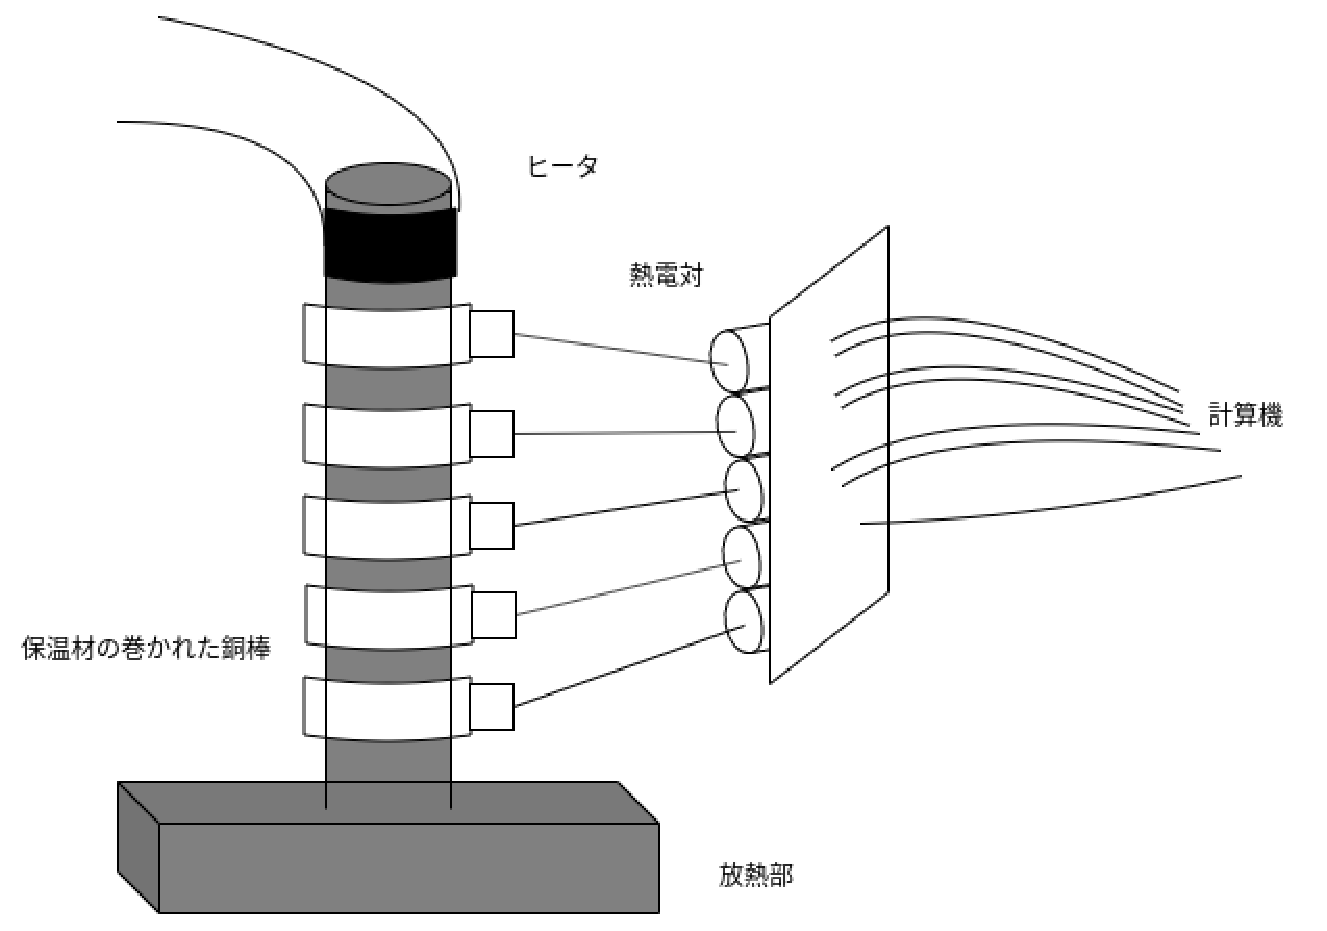
\includegraphics[clip,width=4.0cm]{../Img/FigB1.eps}
%    \label{FigB1}
%  }
%  %
%  \hfill
%  %
%  \subfigure[右側に配置する図の見出し]{
%    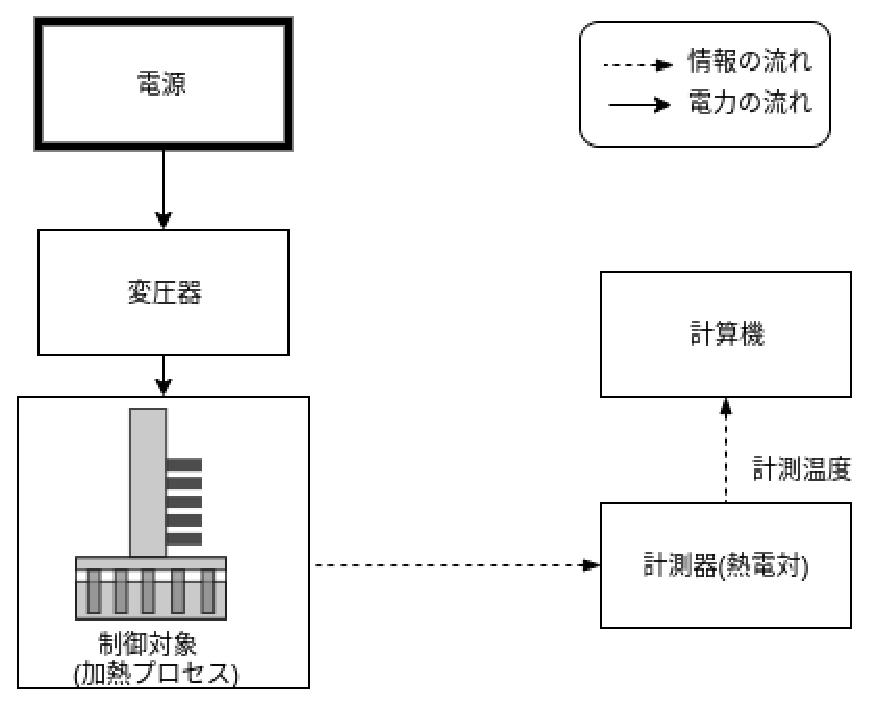
\includegraphics[clip,width=4.0cm]{../Img/FigB2.eps}
%    \label{FigB2}
%  }
%  \end{center}
%  \vspace{-0.5cm}
%  \caption{全体の見出し}
%  \label{図全体へのラベル}
%\end{figure}

\begin{figure}[tb]
  \begin{center}
    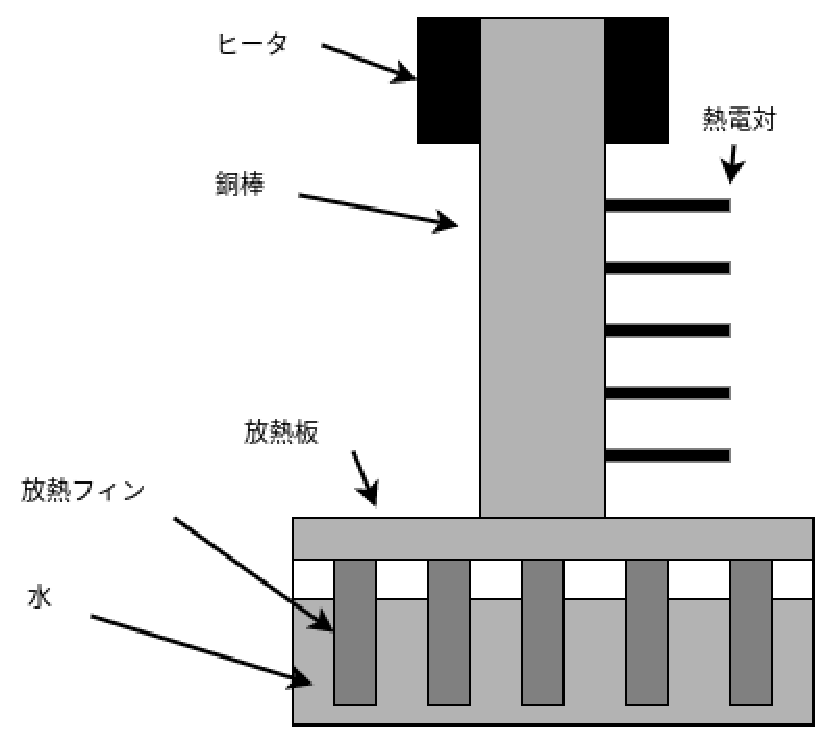
\includegraphics[clip,width=7.0cm]{../Img/FigB3.eps}
    \caption{加熱プロセスの概要}
    \label{FigB3}
  \end{center}
\end{figure}
\subsection{未知パラメータの同定}
 本実験ではステップ応答法により未知パラメータの同定を行う.式(\ref{B3-2})にステップ入力$Q_0(s) = A/s$を加えると,出力は
\begin{equation}
  \label{B3-3}
  \theta(t) = AK_p(1-e^{-(t-L_p)/T_p})
\end{equation}
となる.ここで,$\Delta\theta(t)=\theta(t+h_1)-\theta(t)$($h_1$:データ処理用サンプリング周期)と定義すると,
\begin{equation}
  \label{B3-4}
  \Delta\theta(t) = AK_p(1-e^{-h_1/T_p})e^{-(t-L_p)/T_p}
\end{equation}
となる.さらに$z(t)=ln\Delta\theta(t)$とすると,
\begin{equation}
  \label{B3-5}
  z(t) = -at+b, a = \frac{1}{T_p}, b = ln{AK_p(1-e^{-h_1/T_p})} + \frac{L_p}{T_p}
\end{equation}
となる.すなわち,$z(t)$と$t$の関係(具体的には$a$の値)が分かれば,時定数$T_p$を求めることができる.しかし,$K_p$と$L_p$の値は$b$の値が分かっていても,この条件のみから計算することはできない.そこで$K_p$はシステムのゲイン,すなわち定常状態での入力信号と出力信号の比であるから,次のように考えることができる.
\begin{equation}
  \label{B3-6}
  K_p=\frac{\theta(\infty) - \theta(0)}{A}
\end{equation}
ここで,$\theta(\infty)$は同定実験終了時の定常状態の温度,$\theta(0)$は実験開始前の初期温度,$A$は入力電力であり,式(\ref{B3-6})より$K_p$を計算できる.この結果を式(\ref{B3-5})に代入すれば$L_p$が求められる.以上をまとめると次のようになる.
\begin{description}
  \item[(1)]入力電力を設定し,ステップ応答実験(同定実験)を行う.このとき,初期温度,最終温度を記録しておく.
  \item[(2)]データ処理用サンプリング周期$h_1$の値を定める.
  \item[(3)]実験で得られたデータをプロットする.実験で得られたデータにはノイズが含まれているので,プロットしたグラフをよく観察し,必要に応じて移動平均などの処理を行う.
  \item[(4)]$\Delta\theta(t) = \theta(t+h_1)-\theta(t)$および$z(t)=ln\Delta\theta(t)$を計算し,$t-z(t)$のグラフを作成する.
  \item[(5)]最小二乗法を用いて式(\ref{B3-5})の$a,b$を求め,時定数$T_p$を計算する.$t-z(t)$のグラフは実験初期ではむだ時間部分の影響で,十分時間が経った後は対数の性質により,ばらつきが大きくなるので最小二乗法を用いる範囲には十分注意すること.また,得られた直線を$t-z(t)$のグラフに重ねて描き,計算の妥当性を確認しておく.
  \item[(6)]$K_p$を計算し,$L_p$を求める.
\end{description}
\subsection{最短時間制御系の構成}
\begin{description}
\item[(1)]求めたパラメータを使って,システムの伝達関数を求める.
\item[(2)]最大入力$A_{max}$ = 50[W]を入力した場合と定常入力$A_s$を入力した場合の位相面軌道をそれぞれ描く.なお,むだ時間については考えなくてもよい.
\item[(3)]最短時間制御を行うために,切り替え後の入力電力$A_s$,切り替え時間$T_\omega$を計算する.
\end{description}
\subsection{最短時間制御}
 特定の性能に対しては,非線形動作のほうが線形のものより優秀であることが知られている.ボントリアギンの最大原理によれば,たとえば時間を最短にする制御動作はban-ban型の制御方式をとる.このような制御系を設計する場合には,位相面解析法は直感的にも理解しやすく,図式的に解くのも利用される.\\
 ここでは,実験に沿って,一次遅れ系の最短時間制御について説明する.\\
\begin{table}[tb]
  \begin{center}
    \caption{平衡点の種類}
    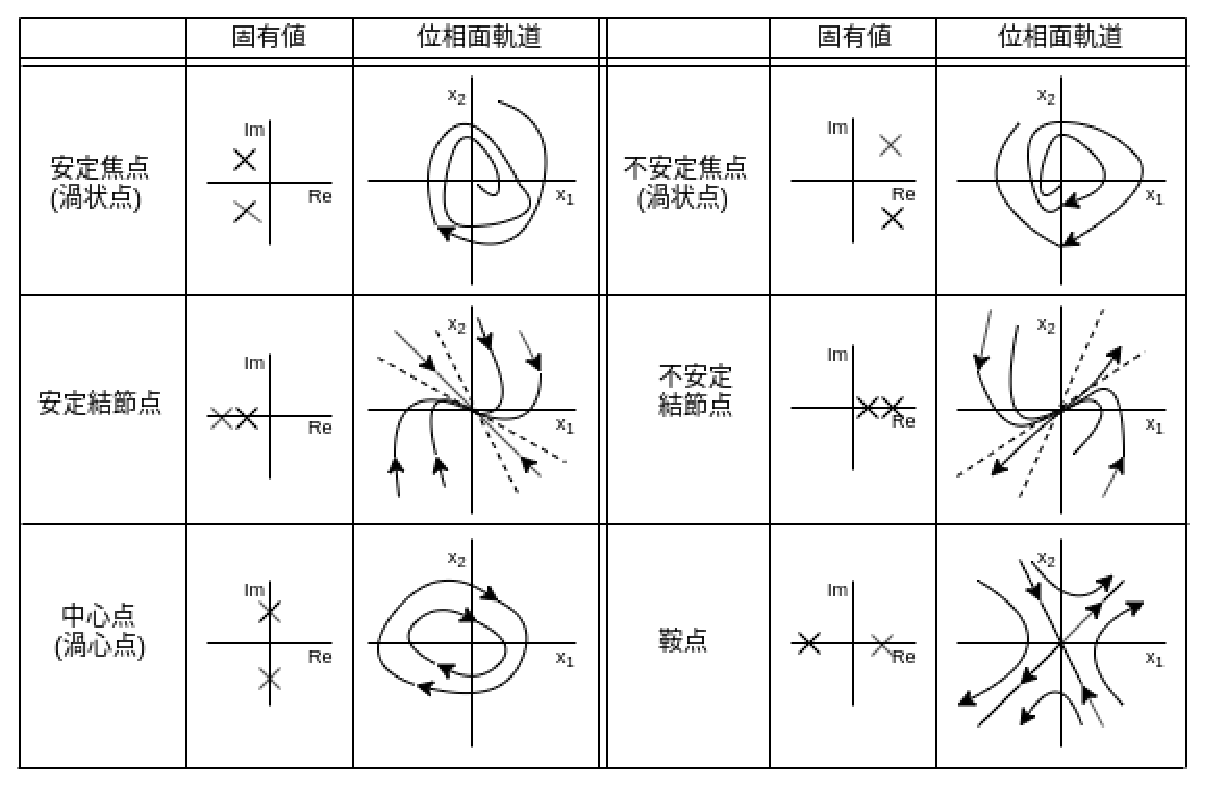
\includegraphics[clip,width=7.0cm]{../Img/FigC1.eps}
    \label{FigC1}
  \end{center}
\end{table}
\begin{figure}[tb]
  \begin{center}
    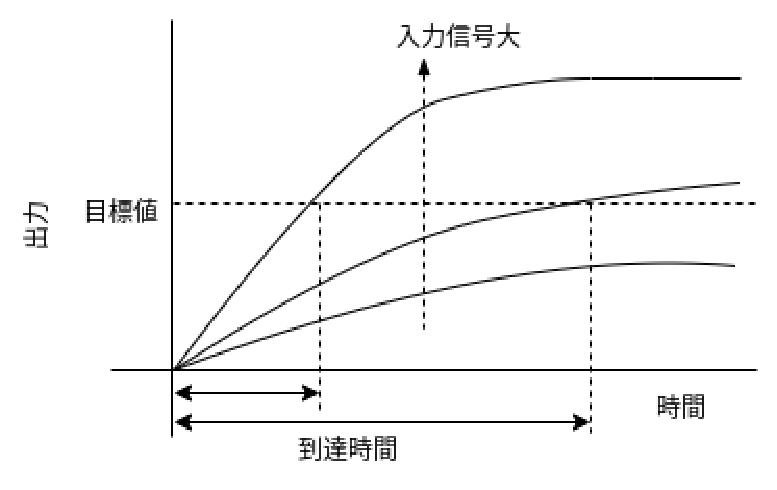
\includegraphics[clip,width=7.0cm]{../Img/FigC4.eps}
    \caption{最短時間制御を実現する入力}
    \label{FigC4}
  \end{center}
\end{figure}
  まず,1次遅れ系の伝達関数は
\begin{equation}
\label{C10}
G_p = \frac{K_p}{1+T_ps}
\end{equation}
で表される.このような系に対し,出力がある値まで最短の時間で到達することを考えよう.どのような入力に対しても,時定数は一定であるから,入力信号のゲインが大きいほど大きいほど,出力がある値に到達する時間は短くなることがわかる.したがって,出力がある値に達するまで,対象となるシステムにおいて許容し得る最大の入力信号を加えるとよい(図\ref{FigC4}).\\
 しかし,このままでは出力がある値まで最短の時間で到達することを最短になるが,出力は定常状態に落ち着くまで増加を続ける.そこで,出力がある値に到達したとき(あるいは到達する前)に,ある値に落ち着くような入力信号に切り替え,制御を達成しようと考える.この切り替えるタイミング(切り替え時間と呼ぶ)と切り替え後の入力を得るために,位相面軌道を使って解析する.\\
 次に,式(\ref{C10})で表される系のステップ応答を考える.入力を$U(s)=A/s$とおくと,そのときの出力は
\begin{equation}
\label{C11}
Y(s) = G_p(s)U(s) = \frac{AK_p}{s(1+T_ps)}
\end{equation}
となる.式(\ref{C11})の両辺に$1+T_ps$を掛け,逆ラプラス変換すると,
\begin{equation}
\label{C12}
y(t) + T_p\dot{y}(t) = AK_p
\end{equation}
が得られ,これを$\dot{y}(t)$について解くと,
\begin{equation}
\label{C13}
\dot{y}(t) = -\frac{1}{T_py(t)} + \frac{AK_p}{T_p}
\end{equation}
\begin{figure}[tb]
  \begin{center}
    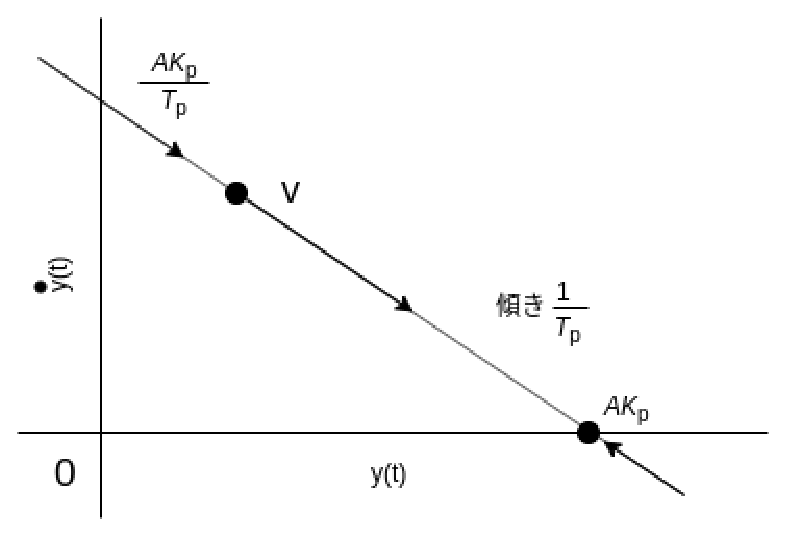
\includegraphics[clip,width=7.0cm]{../Img/FigC5.eps}
    \caption{一次遅れ系のステップ応答の位相面軌道}
    \label{FigC5}
  \end{center}
\end{figure}
が得られる.これは$y(t)$の1次関数であるから,位相面($y(t)-\dot{y}(t)$平面)に軌跡を描くと,図\ref{FigC5}のようになる.\\
 ここで,位相面軌道上の状態の移動方向を考えよう.今,図\ref{FigC5}で直線上の点V(第1象限)に状態があったとする.このとき,この系の移動速度$\dot{y}(t)$は正であるから,変位$\dot{y}(t)$は増加する.したがって,状態は図の矢印の方向に移動することがわかる.また,状態が第四象限にあった場合には,移動速度$\dot{y}(t)$が負であることから,変位$y(t)$は減少し,図の矢印の方向に移動することがわかる.同様に,第二象限,第三象限についても考えることができ,直線上の全ての点は,入力信号の大きさ$A$と制御対象のゲイン$K_p$によって決まる定常値$AK_p$に向かうことがわかる.\\
\begin{figure}[tb]
  \begin{center}
    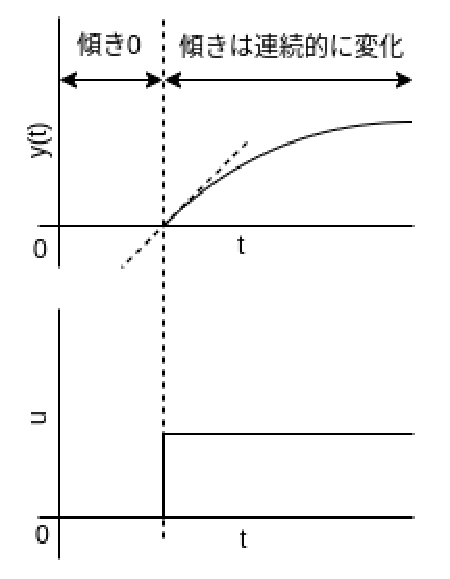
\includegraphics[clip,width=7.0cm]{../Img/FigC6.eps}
    \caption{一次遅れ系のステップ応答}
    \label{FigC6}
  \end{center}
\end{figure}
\begin{figure}[tb]
  \begin{center}
    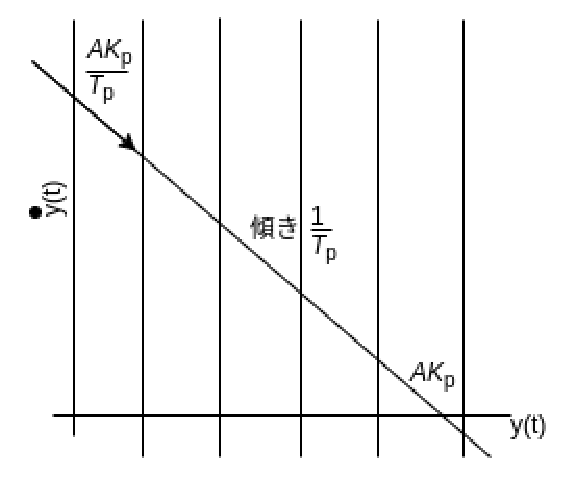
\includegraphics[clip,width=7.0cm]{../Img/FigC7.eps}
    \caption{一次遅れ系のステップ応答の位相面軌道}
    \label{FigC7}
  \end{center}
\end{figure}
\begin{figure}[tb]
  \begin{center}
    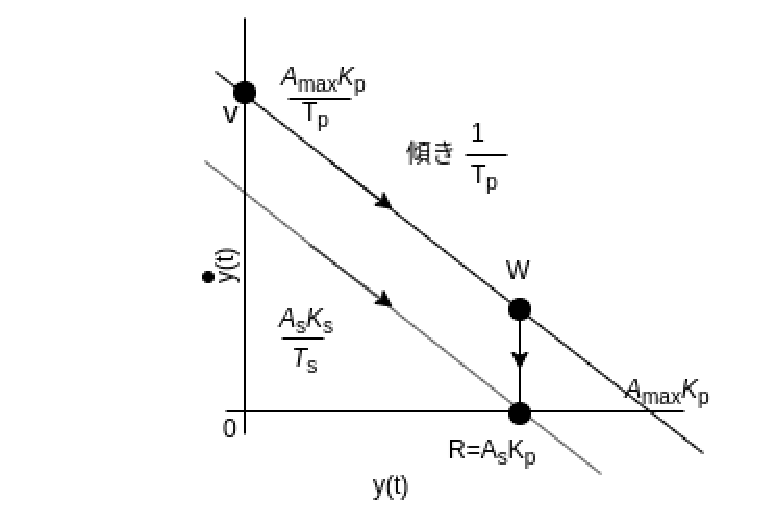
\includegraphics[clip,width=7.0cm]{../Img/FigC8.eps}
    \caption{最短時間応答の位相面軌道}
    \label{FigC8}
  \end{center}
\end{figure}
 ところで,初期状態Vが直線上にない場合はどのような軌道を描くのであろうか.これを明らかにするために,1次遅れ系のステップ応答において,ステップ入力が入力された時点の応答の様子を考えてみよう.図\ref{FigC6}に1次遅れのステップ応答と入力の様子を示す.入力が加わる前は系の応答は一定値,すなわち傾き0の直線となるが,ひとたび入力が加わると系の応答の傾きは不連続的に変化し,0からある有限の値にジャンプすることがわかる.もう少し,一般的に考えて,入力が0の部分でステップ状の入力があったとしても,入力が変化しない間は出力の傾きは連続的に変化し,入力がステップ状に変化したときに出力の傾きが不連続的に変化することが想像できる.傾きが不連続的に変化する状況を位相面上で考えると,変位$y(t)$は一定で速度$\dot{y}(t)$が変化する状況になる.すなわち,位相面上では$\dot{y}(t)$軸に平行な直線となる.\\
 以上のことをまとめると,式(\ref{C10})で表される一次遅れ系に$U(s)=A/s$というステップ入力を加えた場合の任意の点からの位相面軌道は図\ref{FigC7}で表される.\\
 すなわち,ある状態の制御系に対し,ステップ入力を加えた瞬間に式(\ref{C11})で表される直線上に状態は移行し,その後はその直線上を移動する.\\
 前述したように,出力が目標値に最短で到達するには,その系で許容される最大の入力信号を加えればよい.しかし,そのままでは出力は目標値を超えてしまう.そこで,目標値で定常状態となるような入力を加えた場合とその系で許容される最大の入力を加えた場合の位相面軌道を同一の位相面に描いてみよう(図\ref{FigC8}).\\
  初期値は簡単のため位相面の原点とする.目標値へ最短の時間で到達するため,最大ステップ入力$A_{max}$を加えると,状態は点Vから点Wへ向かって移動を始める.状態が点Wへ達した瞬間,すなわち,目標値へ達した瞬間に,入力の大きさを$A_{max}→ A_{s}$へ切り替えると($A_s$は目標値$R$で定常となるようなステップ入力),図\ref{FigC7}をみるとわかるように,状態は$\dot{y}(t)$軸に平行に移動し目標値$R$で定常状態に落ち着くと予想される.図\ref{FigC7}の説明のところで述べたように,一次遅れ系においては入力がステップ状に変化したとき,出力の傾きは瞬時に変化するから,図のW-R間の所要時間は0である.また,位置0からRまで変化するのに要する時間は直線VW,すなわち,入力$A_{max}$を加えたときがもっとも短い.したがって,出力を最短時間で目標値Rに整定させるには0-V-W-Rの経路を通るような入力を加えればよいということがいえる.\\
  このような経路を通るような入力はどのような形になるのか.ここでは,経路を二つに分けて考えよう.すなわち,最大許容入力$A_{max}$を加え,目標値に最短で達するまで(0-V-W)と,目標値に達した後(W-R)の部分である.点Wまでは最大ステップ入力$A_{max}$を加えた状態であるから,最短時間応答を実現する入力を以下のようにおく.\\
\begin{equation}
  \label{C14}
  u(t)=A_{max}×1(t) + \dot{u}(t)
\end{equation}
式(\ref{C14})で$\dot{u}(t)$の形を決定すれば,求める入力が得られる.\\
 先程も述べたように,点Wまでは最大ステップ入力$A_{max}$を加えた状態であるから,点Wに到達する時間を$T_W$とおくと,$0<t<T_W$では$\dot{u}(t)=0$.$T_W<t$では$u(t)=A_S×1(t)$だから,
\begin{equation}
  \label{C15}
  u^{\prime}(t)=(A_S-A_{max})1(t)
\end{equation}
となる.したがって,以上をまとめると,
\begin{equation}
  \label{C16}
  u(t)=A_{max}×1(t)+(A_S-A_{max})1(t-T_W)
\end{equation}
となる.すなわち,制御開始後$T_W$秒間は最大入力$A_{max}$を入力し,時刻$T_W$秒で入力の大きさを$A_S$に切り替えることで最短時間制御が実現できる.\\
 切り替え時間$T_W$はV-W間の経過時間を計算すればよい.速度$\dot{y}(t)$は
\begin{equation}
  \label{C17}
  \dot{y}(t)=\frac{dy(t)}{dt}
\end{equation}
であるので,変数分離
\begin{equation}
  \label{C18}
  dt = \frac{1}{\dot{y}}dy
\end{equation}
を行い,両辺を0からRまで積分すると,
\begin{eqnarray}
  \label{C19}
  T_W & = & \int_0^{T_W} dt = \int_0^R \frac{1}{\dot{y}(t)} dy = \int_0^R \frac{T_p}{-y+AK_p} dy\\
  & = & -[T_p ln|-y+AK_p|]^R_0\\
  & = & -T_p(ln|AK_p-R|-ln|AK_p|)
\end{eqnarray}
となり,切り替え時間$T_W$が計算できる.
\section{実験方法}
\subsection{実験準備}
以下の手続きに従って実験の準備を行った.これらの手続きは同定実験と制御実験に共通である.
\begin{description}
  \item[(1)]計算機および実験装置の電源を入れた.
  \item[(2)]電力計の目盛りが0[W]を指しており,加熱プロセスに電力が供給されていないことを確認した.もし電力計の目盛りが0[W]でなかったら,すみやかに変圧器を調整し,供給電力を0[W]にする.
  \item[(3)]A/D変換器操作ソフトを起動した.
  \item[(4)]A/D変換器操作ソフトの各種設定を行った.
\end{description}
\subsection{同定実験(一週目)}
以下の手順に従って同定実験を行った.
\begin{description}
  \item[(1)]起動したA/D変換器操作ソフトのウィンドウ上部のサンプリング開始ボタンを押し,速やかに供給電力を50[W]に調整した.
  \item[(2)]ディスプレイに温度計測の時間経過および温度グラフが表示されるので,正常に計測されていることを確認した.
  \item[(3)]各チャネルの温度が約2時間後に定常状態に収束したら,供給電力を0[W]に調整し計測を続けた.
  \item[(4)]計測温度の下降が収束して定常状態となったら,A/D変換器操作ソフトのウィンドウ上部のサンプリング停止ボタンを押した.または,計測時間が3時間に達した場合には,自動的に計測が終了する.「関数によりサンプリングが停止しました」というウィンドウが表示されるので「OK」をクリックした.
  \item[(5)]データ保存ボタンをクリックして計測データを保存した.保存ファイル名は「各班名」とし,ファイルの種類は「Microsoft Excelファイル(*.xls)」を選択した.
  \item[(6)]データを印刷し実験を終了した.
\end{description}
\subsection{計算(二週目)}
\begin{description}
  \item[(1)]3.2節を参考にして,各チャネルごとに未知パラメータを導出した.
  \item[(2)]求めたパラメータを用いて,伝達関数から微分方程式を解き,50[W]のステップ入力に対する時間応答を描いた.一週目の実験で得られた制御対象の応答と比較し,求めたパラメータが妥当であることを確認した.
  \item[(3)]最短制御を参考にして計算したパラメータをもとに切り替え時間および切り替え後の入力電圧値を求めた.
\end{description}
\subsection{制御実験}
\begin{description}
  \item[(1)]A/D変換器操作ソフトによって全チャネルの温度が計測されるので,制御しようとするチャネルの初期温度を以下の手順に従って計測し記録した.
  \begin{description}
    \item[(a)]サンプルスタートボタンをクリックし計測を開始した.
    \item[(b)]表示される各チャネルの温度のグラフから制御対象のチャネルの温度が制御可能な範囲に入っていることを確認した.
    \item[(c)]ウィンドウ右下に表示される「Status」ボタンをクリックした.
    \item[(d)]このボタン上部に表示される「Status表示ウィンドウ」上部の「CH」から制御対象のチャネルを選択した.
    \item[(e)]「カーソル」表示にY:・・・[V]と電圧が表示された.
    \item[(f)](a)から(e)操作をくり返し,制御対象のチャネルの温度が制御可能範囲にあることを確認すると同時に,そのときの温度を初期温度として記録した.
  \end{description}
  \item[(2)]前の手順で測定した初期温度と目標温度,同定実験で求めたパラメータをもとに,3.3節を参考にして切り替え時間$T_{\omega}$,定常入力$A_S$を計算した.このとき,初期値は0ではなく,測定した初期温度になるので注意する.
  \item[(3)]計算した切り替え時間および定常入力(切り替え後の入力)を入力した.一人は供給電力を調整できるように準備する.
  \item[(4)]ディスプレイに温度計測の時間経過が表示されるので,すみやかに供給電力が50[W]になるように調整し,正常に計測されていることを確認した.切り替え時間は,表示画面の右下に表示される時間(ms)を確認しながら,設定した定常入力に調整できるよう準備した.
  \item[(5)]切り替え時間になると同時に,設定した定常入力電力になるように電圧制御装置を調整した.
  \item[(6)]温度が安定したら,サンプリング停止ボタンをクリックした.「関数によりサンプリングが停止しました」という画面が出てくるので「OK」をクリックした.
  \item[(7)]データ保存ボタンをクリックして計測データを保存した.その際,ファイル名は「各班名」とし,ファイルの種類は「Microsoft Excelファイル(*.xls)」を選択すること.必要ならば結果を印刷し実験を終了した.
  \item[(8)]次の実験を行うために,備え付けの扇風機等を用いて加熱棒の温度を初期温度付近まで下げた.温度が安定したら,次の実験者が別のチャネルで実験を行った.
\end{description}
\section{実験結果}
チャネル5を使用して制御系の設計を行った.
\subsection{同定実験の結果}
得られたグラフを図\ref{identification_EXP}に示す.
\begin{figure}[tb]
  \begin{center}
    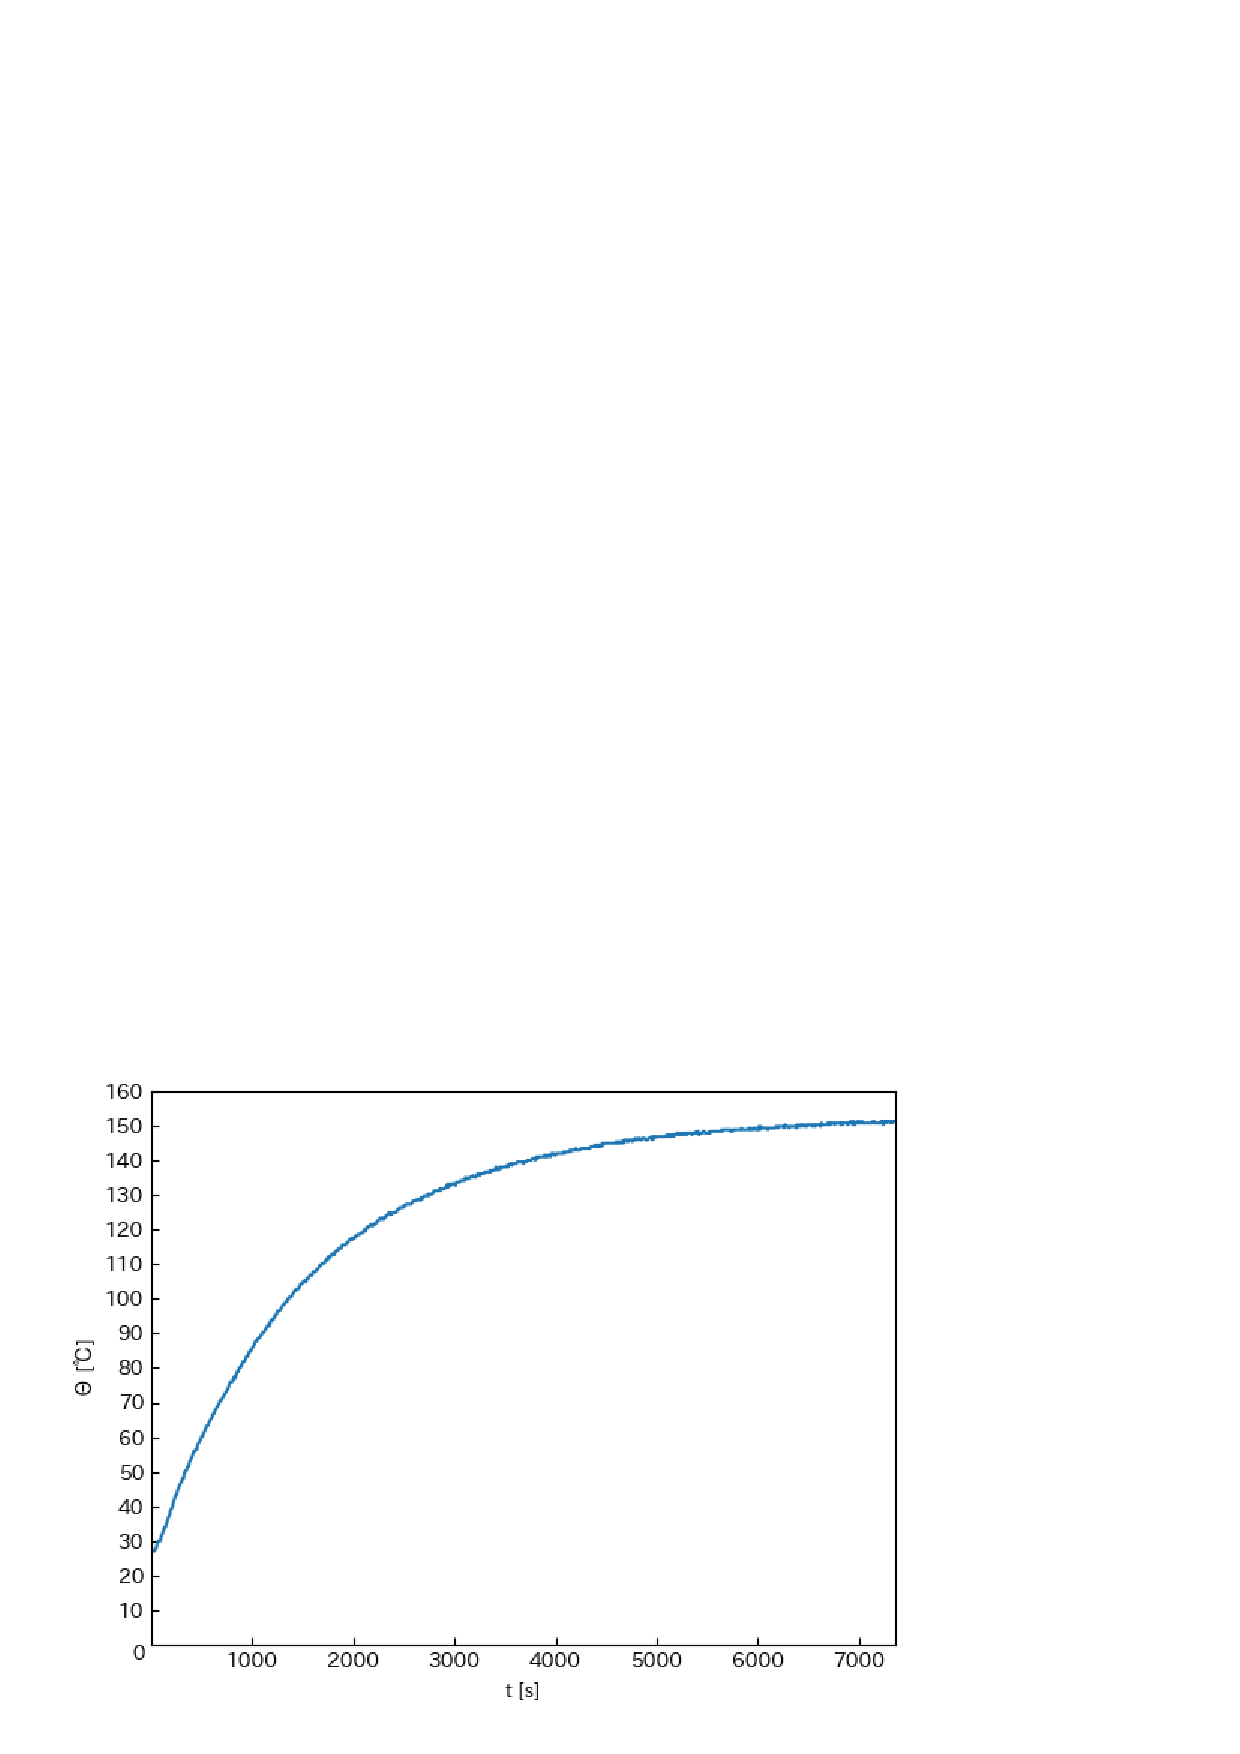
\includegraphics[clip,width=7.0cm]{../graph/identification.png}
    \caption{同定実験により得られたグラフ}
    \label{identification_EXP}
  \end{center}
\end{figure}

\subsection{計算実験の結果}
%\comment{移動平均法}
実験ではデータの平滑化のために移動平均法を使用した.データが激しく変動して,全体的な動きをつかまえにくい場合,細かな変動をならし,傾向線を求める考え方が移動平均の考えである.データを,傾向変動と偶然変動の和と見る.偶然変動を除いて,全体のトレンド傾向を見たい場合に使う.一般に,移動平均は,周期が移動平均の項数に等しい周期的変動を除去してデータを円滑化する\cite{moving_average}.

最小二乗法は,計測点が$X$のとき,$Y$と関数値$f(X)$との差$(Y-f(X))$を計算する.差の2乗$(Y-f(X))^2$が小さければ,$Y$と$f(X)$は近い値となる.差の2乗を全ての点で合計し,その合計値を最小にする.
\begin{equation}
  \label{minimum_required_method}
  T = \sum_{}^{}(Y-f(X))^2
\end{equation}
式(\ref{minimum_required_method})の$T$(合計)が最小となる関数の係数を求める.係数が求まると,任意の$X$での$f(X)$が求まる\cite{minimum_method}.
ここで,関数$y = a + bx_n$とすると,
\begin{eqnarray}
  \label{minimum_method}
  aN + b\sum_{n}^{}x_n = \sum_{n}^{}y_n \\
  a\sum_{n}^{}x_n + b\sum_{n}^{}x_n^2 = \sum_{n}^{}x_ny_n
\end{eqnarray}
となる.これを連立方程式としてとくと,
\begin{eqnarray}
a = \frac{\sum{}^{}y \sum{}^{}x^2 - \sum{}^{}xy\sum{}^{}x^2}{N\sum_{}^{}x^2 - (\sum_{}^{}x)^2}\\
b = \frac{N\sum{}^{}xy - \sum{}^{}x\sum{}^{}y}{N\sum_{}^{}x^2 - (\sum_{}^{}x)^2}
\end{eqnarray}
と求められる.

$h_1=200$[s],$h_1=290$[s],$h_1=300$[s]とし,$z-t$のグラフを図\ref{z-t_h1=200s},図\ref{z-t_h1=290s},図\ref{z-t_h1=300s}に示す.
\begin{figure}[tb]
  \begin{center}
    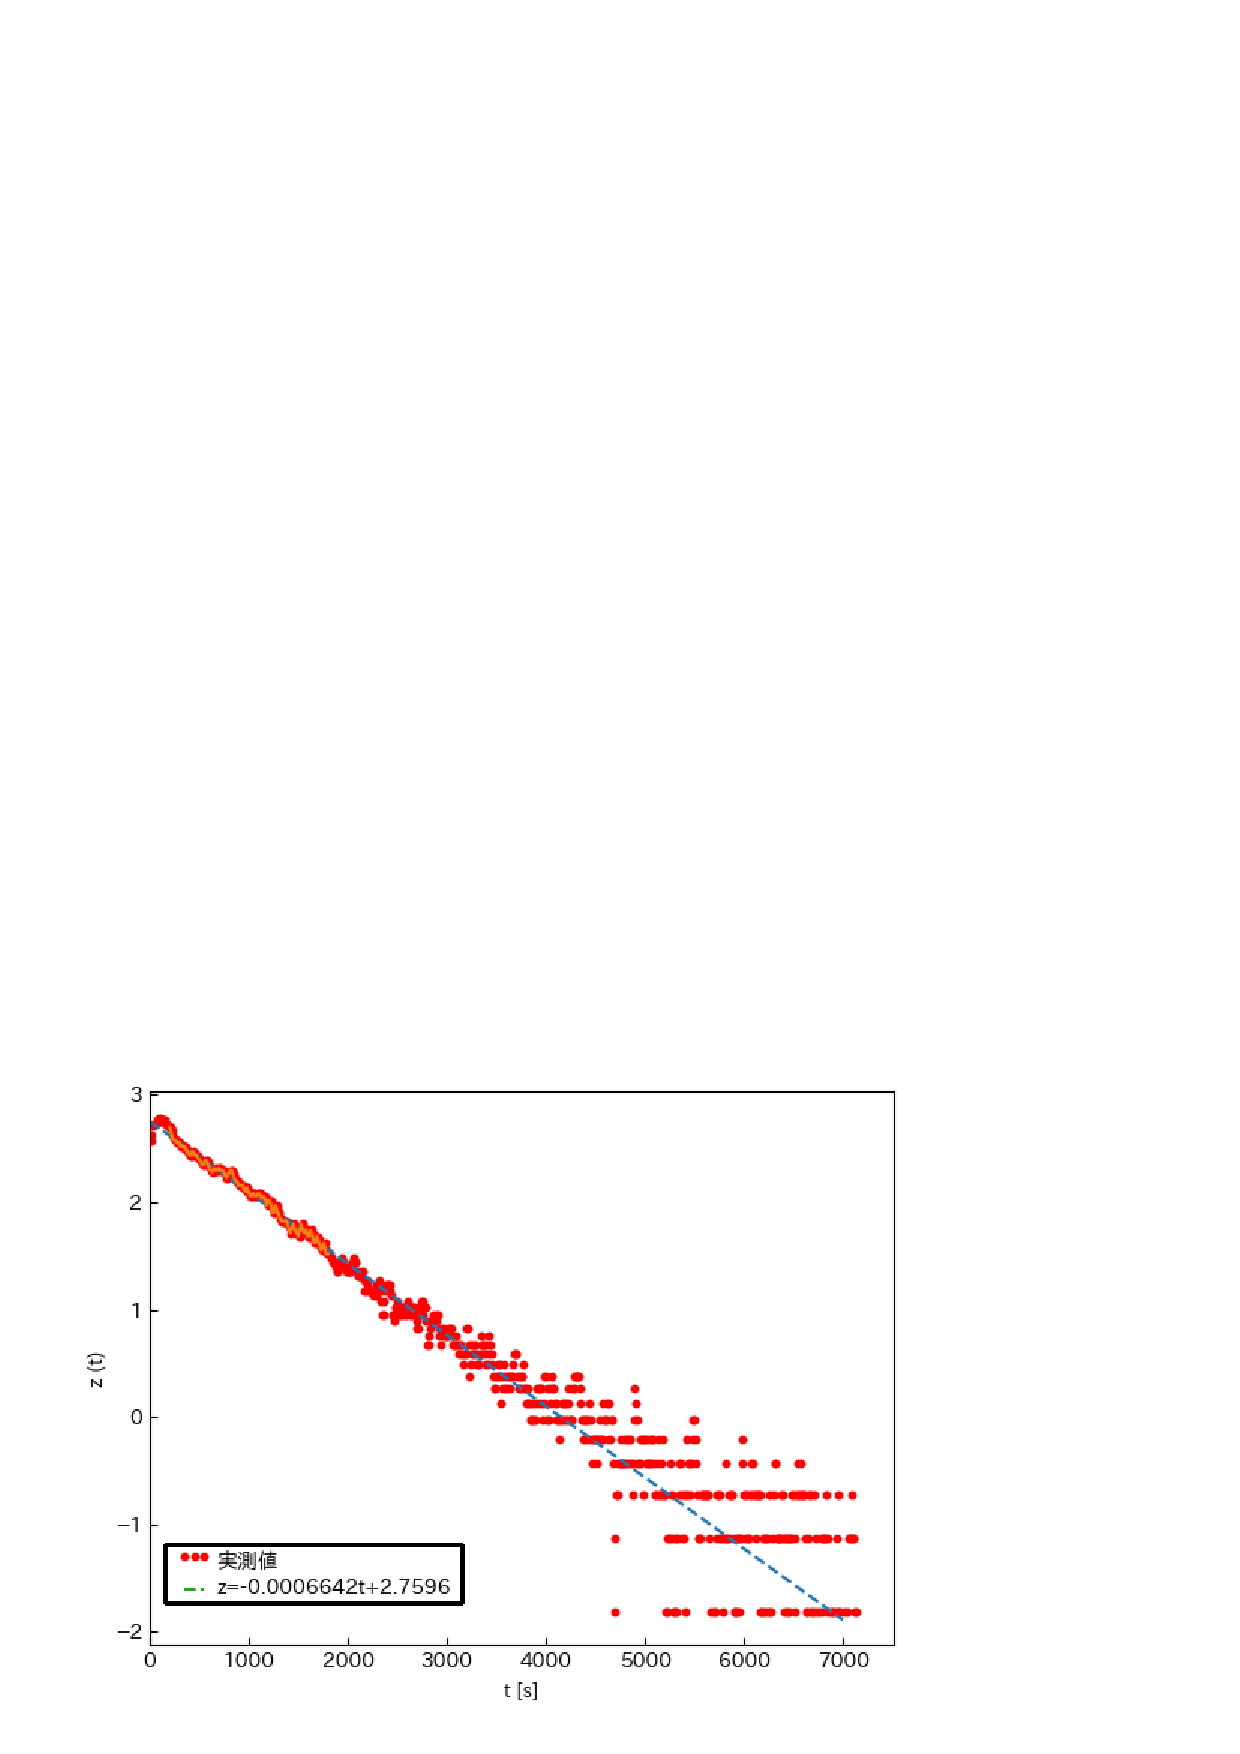
\includegraphics[clip,width=7.0cm]{../graph/z-t200s.png}
    \caption{サンプリング周期200[s]とした時のz-tのグラフ}
    \label{z-t_h1=200s}
  \end{center}
\end{figure}
\begin{figure}[tb]
  \begin{center}
    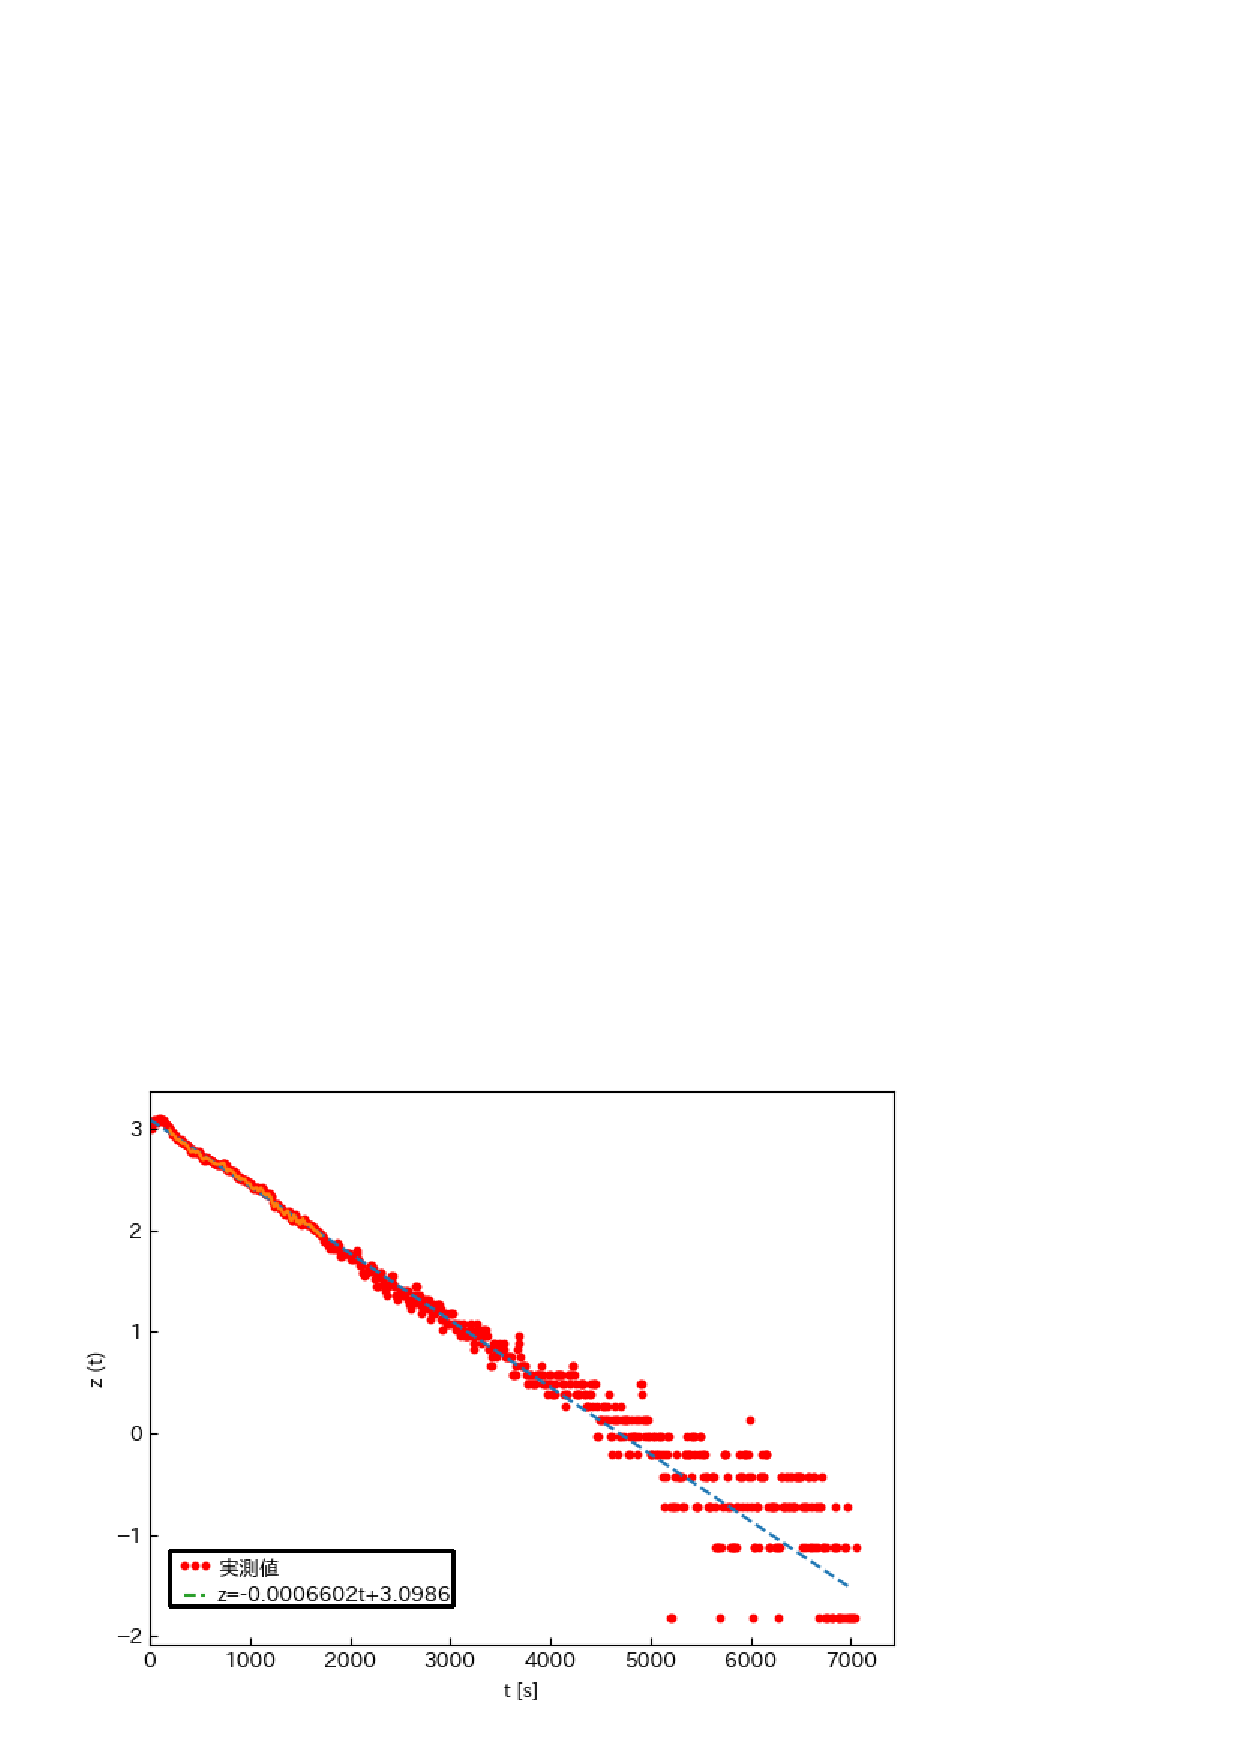
\includegraphics[clip,width=7.0cm]{../graph/z-t290s.png}
    \caption{サンプリング周期290[s]とした時のz-tのグラフ}
    \label{z-t_h1=290s}
  \end{center}
\end{figure}
\begin{figure}[tb]
  \begin{center}
    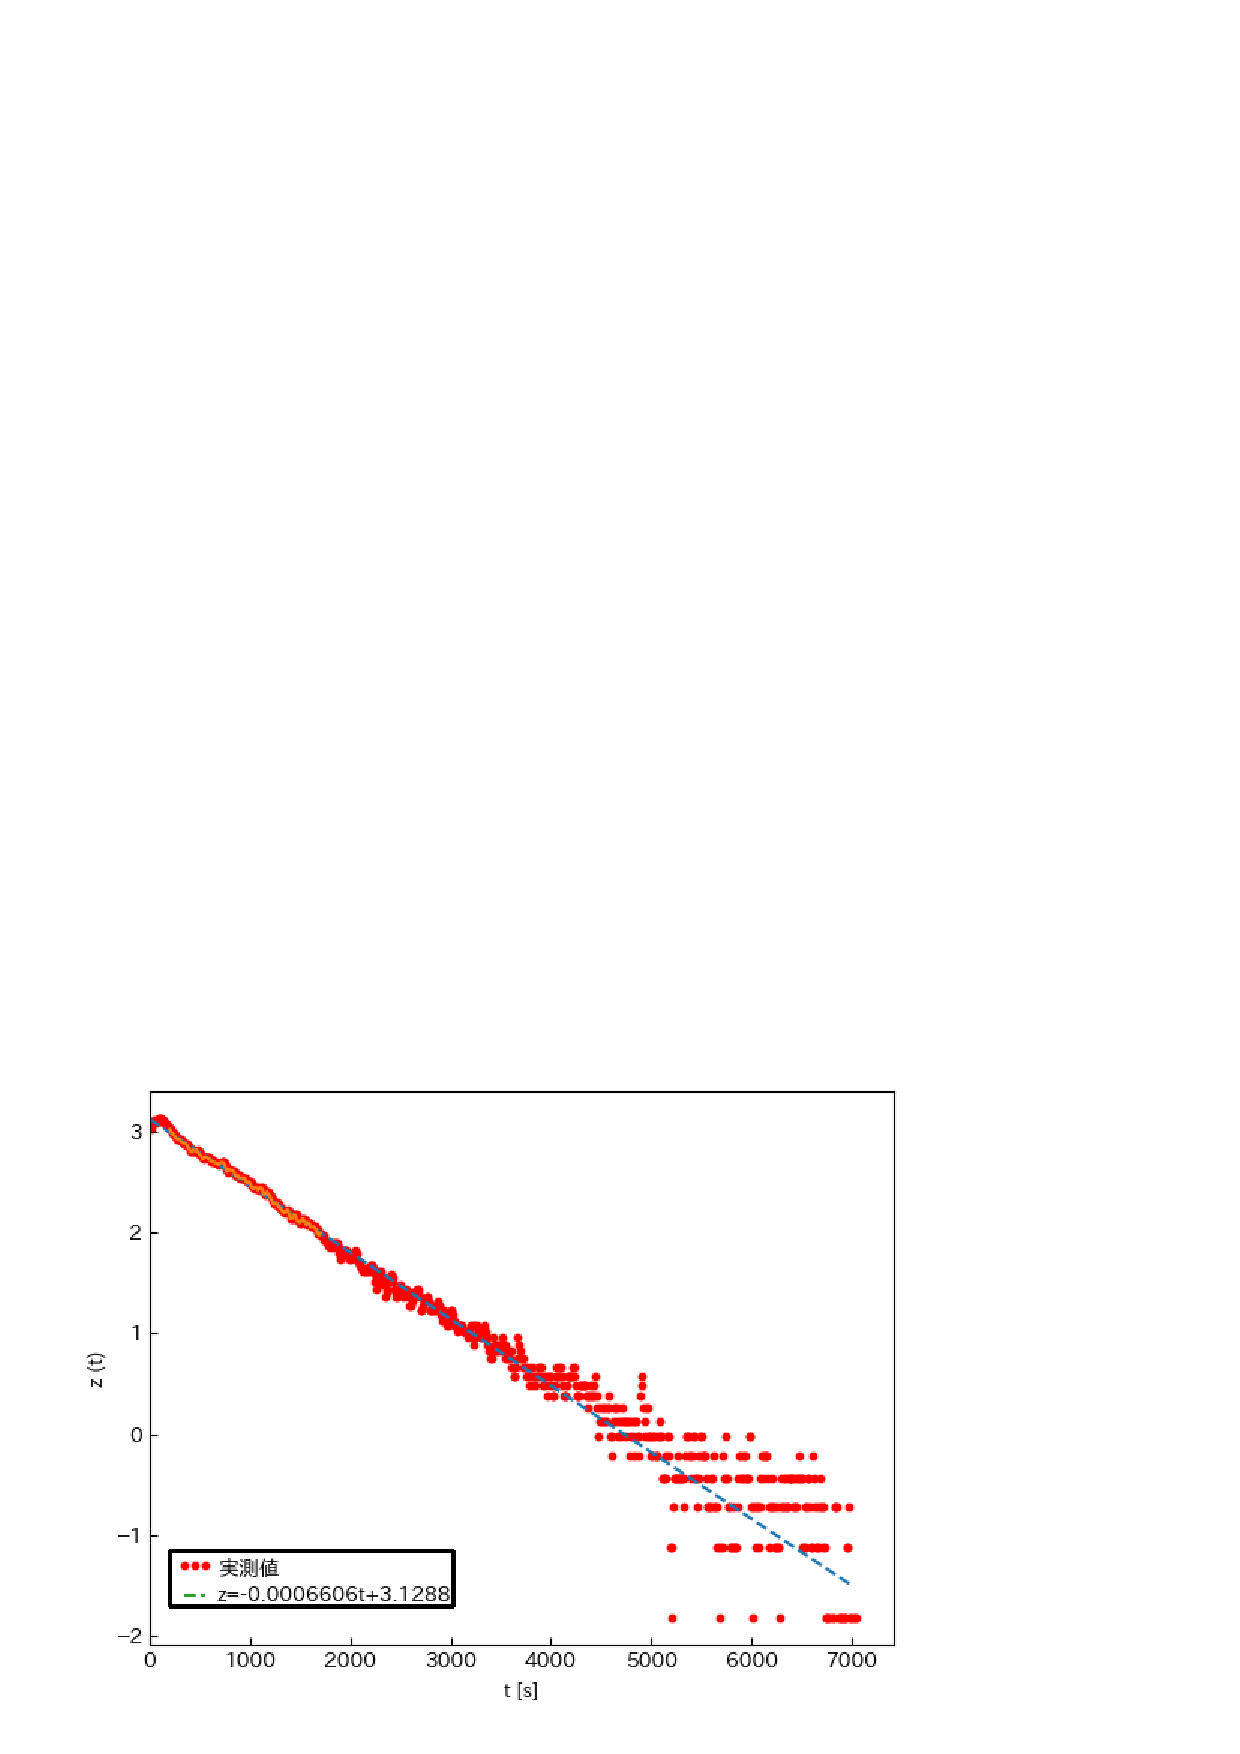
\includegraphics[clip,width=7.0cm]{../graph/z-t300s.png}
    \caption{サンプリング周期300[s]とした時のz-tのグラフ}
    \label{z-t_h1=300s}
  \end{center}
\end{figure}
それらの$a$,$b$の値を使ってパラメータを計算し,ステップ応答の結果を図\ref{step_response200s},図\ref{step_response290s},図\ref{step_response300s}に示す.
\begin{figure}[tb]
  \begin{center}
    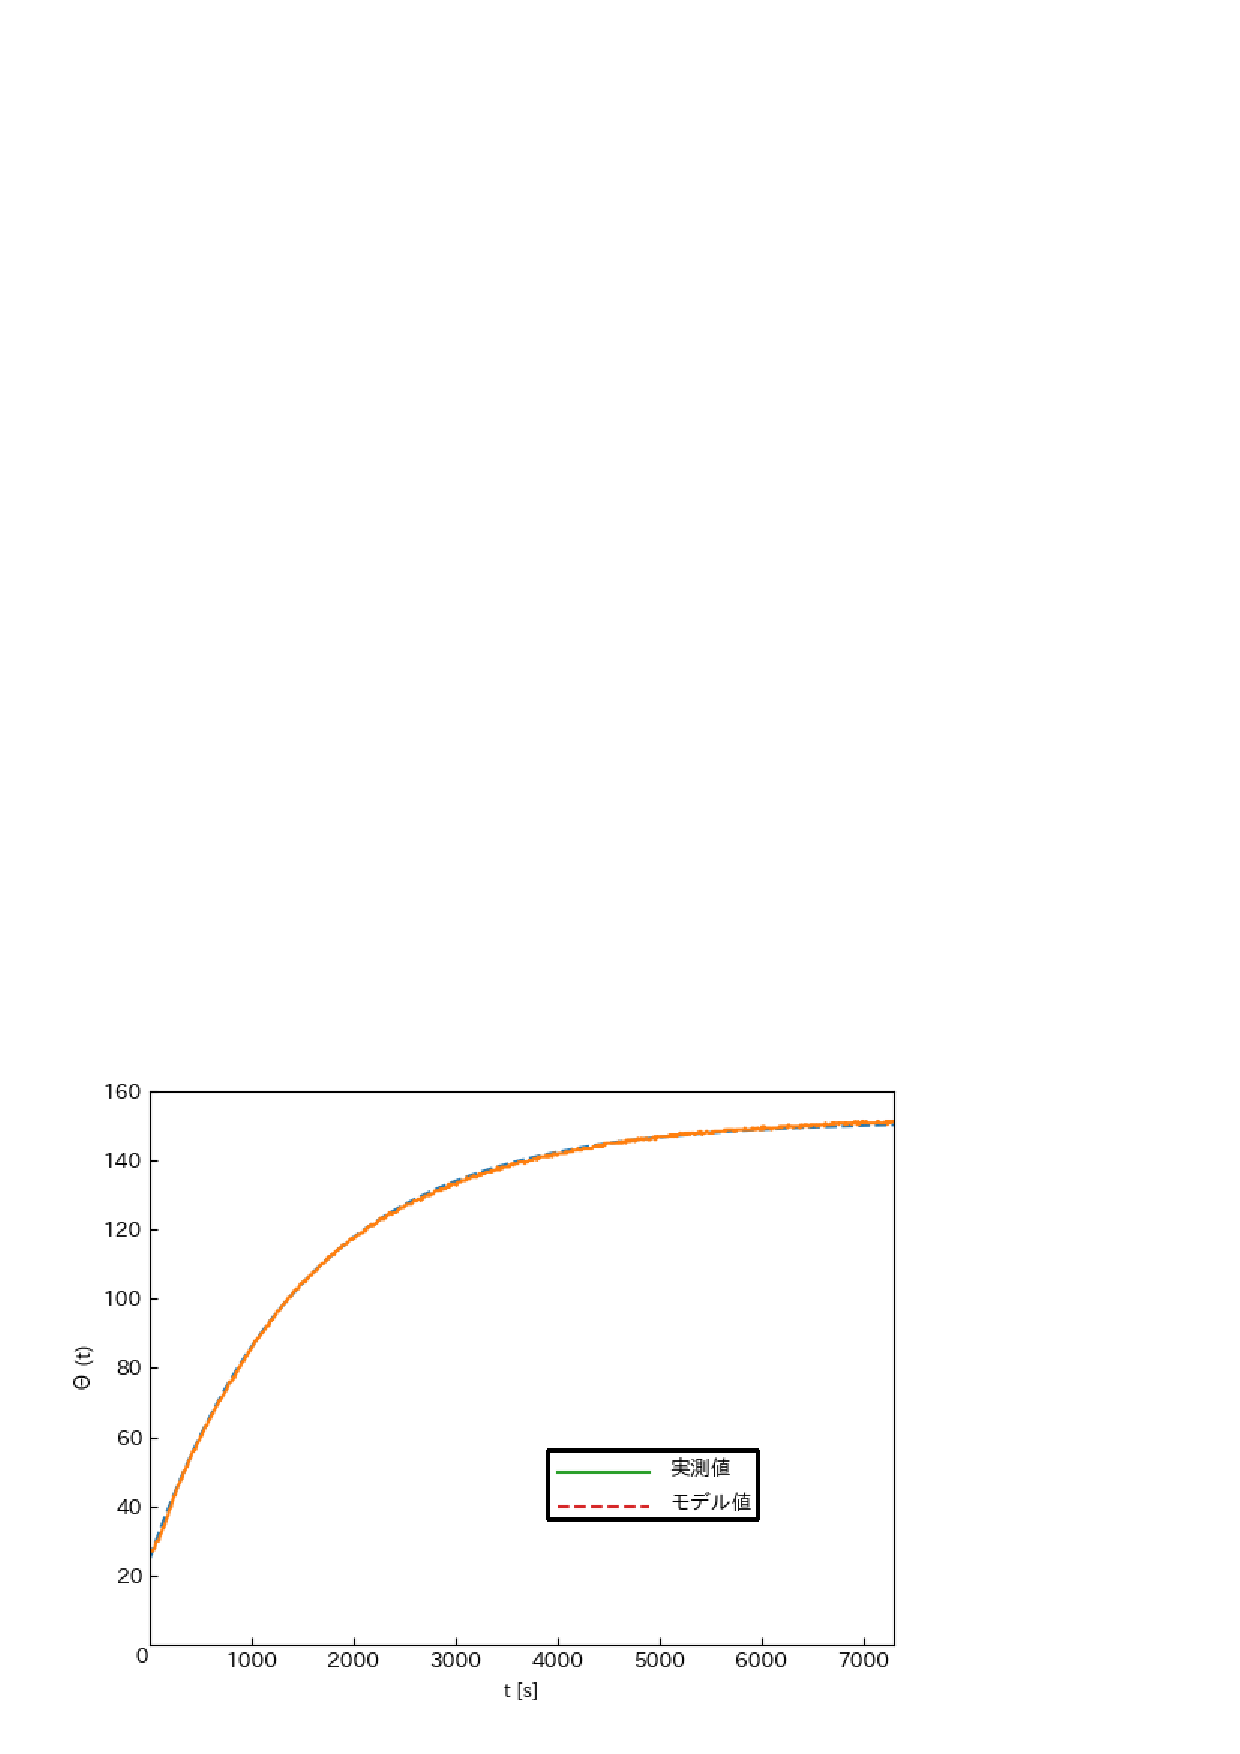
\includegraphics[clip,width=7.0cm]{../graph/step_response200s.png}
    \caption{サンプリング周期200[s]とした時のステップ応答のグラフ}
    \label{step_response200s}
  \end{center}
\end{figure}
\begin{figure}[tb]
  \begin{center}
    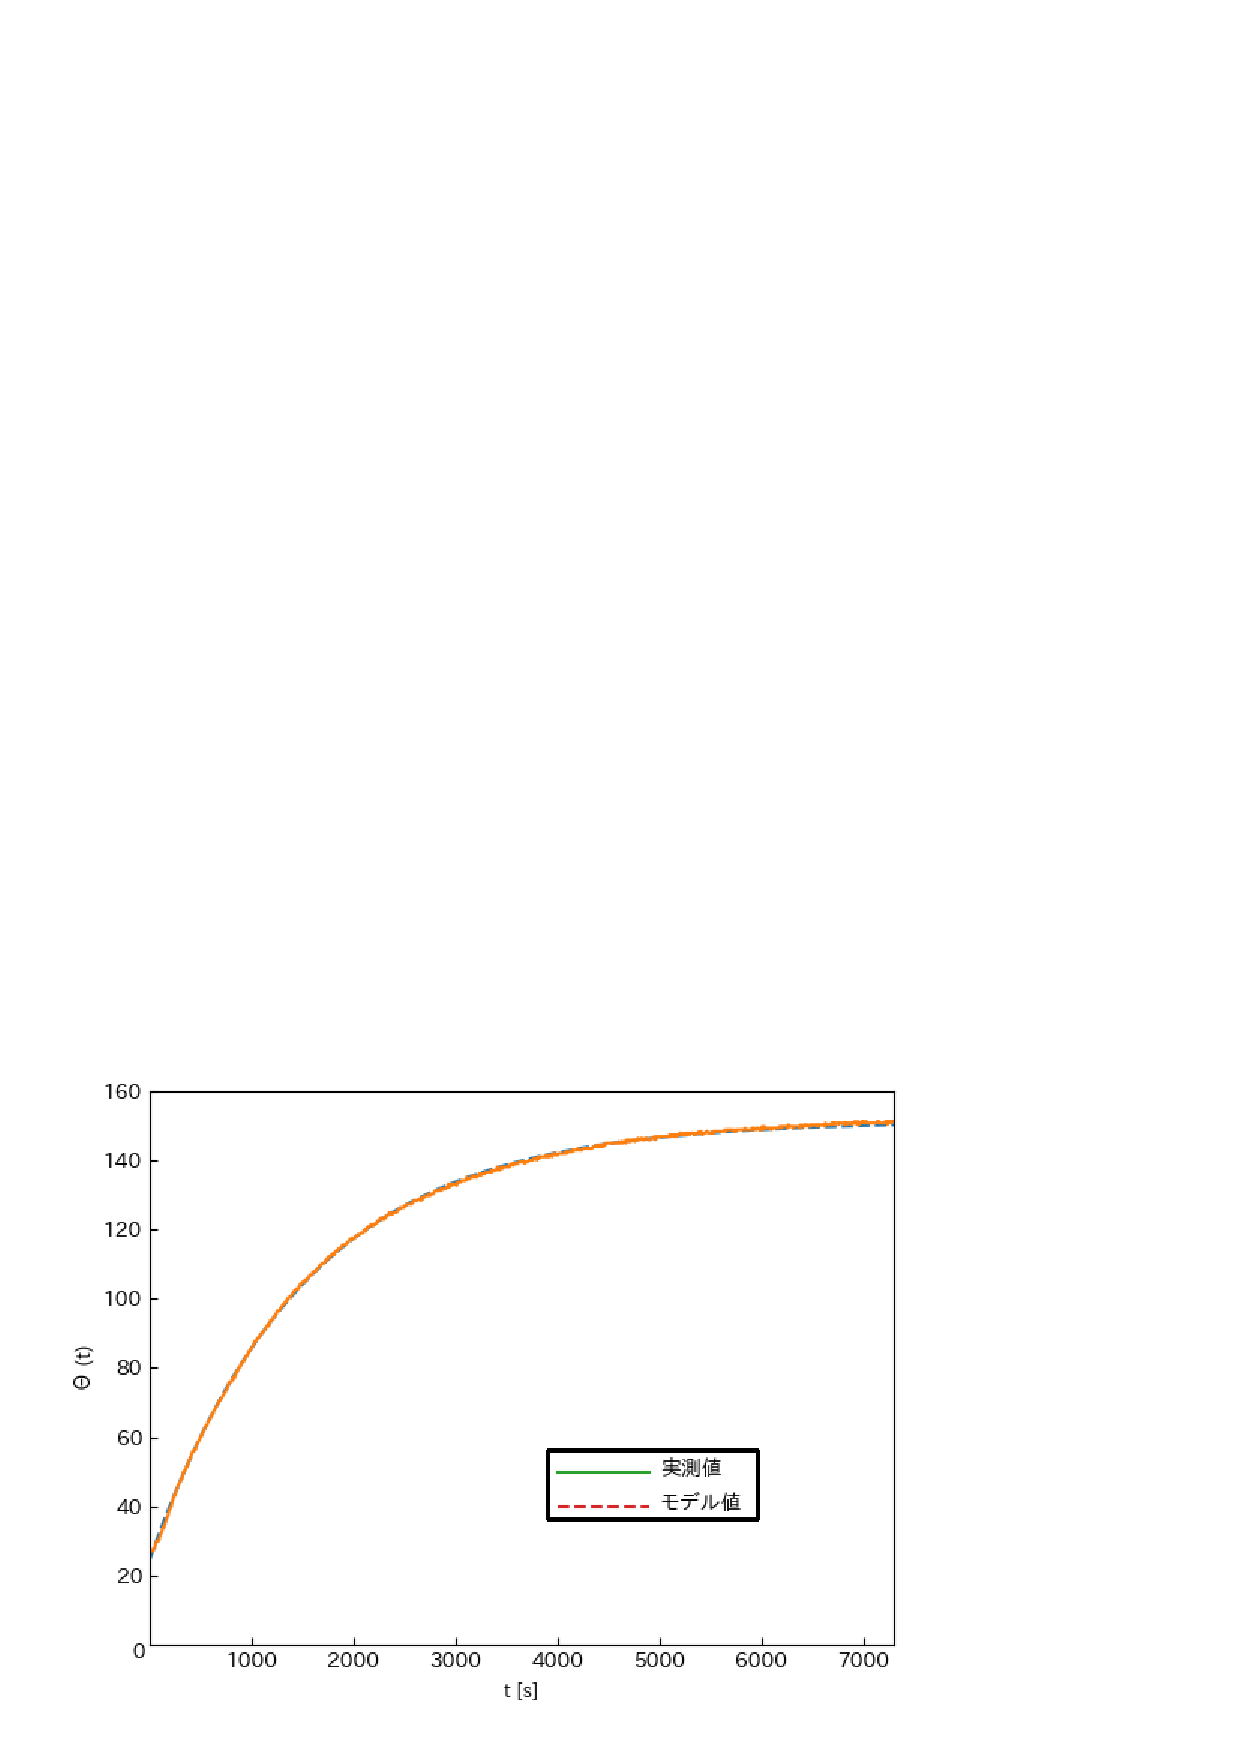
\includegraphics[clip,width=7.0cm]{../graph/step_response290s.png}
    \caption{サンプリング周期290[s]とした時のステップ応答のグラフ}
    \label{step_response290s}
  \end{center}
\end{figure}
\begin{figure}[tb]
  \begin{center}
    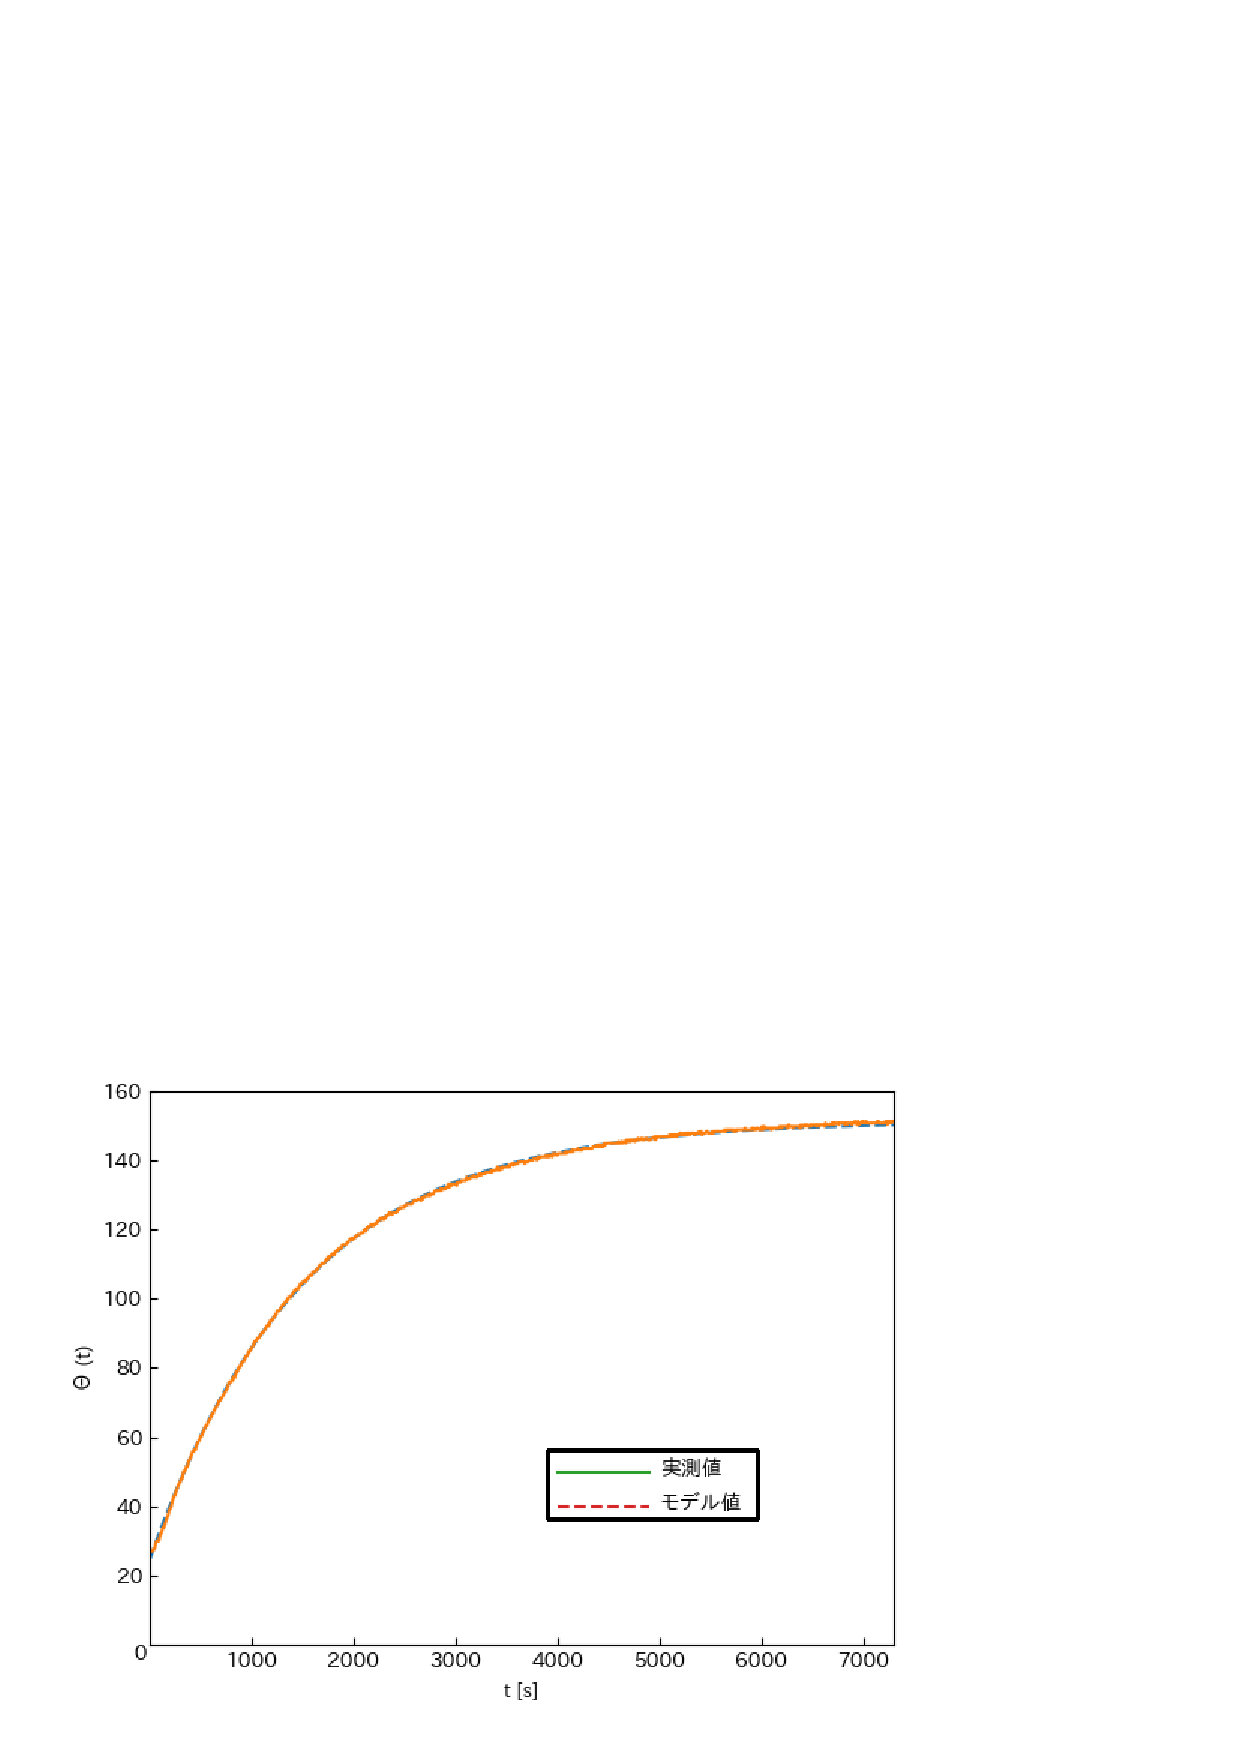
\includegraphics[clip,width=7.0cm]{../graph/step_response300s.png}
    \caption{サンプリング周期300[s]とした時のステップ応答のグラフ}
    \label{step_response300s}
  \end{center}
\end{figure}
求めたパラメータを表\ref{Experiment_ab}にまとめる.
\begin{eqnarray}
  \label{K_p}
  K_p &=& \frac{100 \theta(\infty)- 100 \theta(0)}{A} \\
      &=& 2.490842
\end{eqnarray}
\begin{table}[tb]
  \label{Experiment_ab}
  \caption{計算結果}
  \begin{tabular}{|c|c|c|c|c|c|c|} \hline
    $h_1$ & 適用範囲[s] & $a$ & $b$ & $T_p$ & $L_p$ & $E$[\%] \\ \hline \hline
    200 & 200-2000 & 0.0006642 & 2.7596 & 1505.5348 &  28.9427 & 0.54 \\ \hline
    290 & 200-2000 & 0.0006602 & 3.0986 & 1514.6752 &  32.5544 & 0.42 \\ \hline
    300 & 200-2000 & 0.0006606 & 3.1288 & 1513.7651 &  32.1814 & 0.43 \\ \hline
  \end{tabular}
\end{table}
実験結果の表\ref{Experiment_ab}から,最小の相対誤差を取ったサンプリング周期$h_1=290$[s]を使った結果を採用する.
モデルの伝達関数は次のようになる.
\begin{equation}
  \label{transform_result}
  G(s) = \frac{2.490842}{1+1514.6752s}e^{-32.5544s}
\end{equation}

\subsection{制御実験の結果}
$R=35$[℃]とする.このとき,切り替え時間$T_w$,定常入力$A_s$は次のようになる.
\begin{eqnarray}
  \label{T_w}
  T_w &=& -T_p (ln|A K_p - R| - ln| A K_p|) \\
      &=& 499.8
\end{eqnarray}

\begin{eqnarray}
  \label{A_s}
  A_s &=& \frac{R}{K_p} \\
      &=& 14.1
\end{eqnarray}
初期温度は$\theta(0)=$24.15[℃]であり,
\begin{eqnarray}
  \label{}
  \theta(\infty) &=& \theta(0) + R\\
  &=& 59.15
\end{eqnarray}

実験結果を図\ref{Control_Exp}に示す.
\begin{figure}[tb]
  \begin{center}
    \includegraphics[clip,width=7.0cm]{../graph/Control_Exp.png}
    \caption{最短時間制御の結果}
    \label{Control_Exp}
  \end{center}
\end{figure}

\section{課題と考察}
\begin{description}
\item[(1)]最短時間制御の構成において,むだ時間を考慮しなくてもよい理由を考えよ.\\
最短時間制御の構成において,伝達関数を次のように定める.
\begin{equation}
  \label{transform_useless_time}
  G_p(s) = \frac{K_p}{1+T_ps} e^{-L_ps}
\end{equation}
このとき式(\ref{transform_useless_time})で表される系のステップ応答を考える.入力を$U(s)=A/s$とおくと,そのときの出力は
\begin{equation}
  \label{Ys_useless_time}
  Y(s) = G_p(s)U(s) = \frac{AK_p}{s(1+T_ps)} e^{-L_ps}
\end{equation}
となる.式(\ref{Ys_useless_time})の両辺に$(1+T_ps)$を掛け,逆ラプラス変換すると
\begin{equation}
  y(t) + T_p\dot{y}(t) = AK_pu(t-L_p)
\end{equation}
が得られ,これを,$\dot{y}(t)$について解くと,
\begin{equation}
  \dot{y}(t) = -\frac{1}{T_p}y(t) + \frac{AK_p}{T_p}u(t-L_p)
\end{equation}
が得られる.この式の右辺第2項については,$t < L_p$においては$\frac{AK_p}{T_p}u(t-L_p)=0$であるため,$t < L_p$において次の式を満たす.
\begin{equation}
  \dot{y}(t) = -\frac{1}{T_p}y(t)
\end{equation}
ここで,$y(t)$の初期値は$y(0)=0$なので,$t < L_p$においては$\dot{y}(t)=0$となる.
$t > L_p$においては次の式を満たす.
\begin{equation}
  \dot{y}(t) = -\frac{1}{T_p}y(t) + \frac{AK_p}{T_p}
\end{equation}
よって,位相面($y(t) - \dot{y}(t)$)に軌跡を描くと,むだ時間を考慮しないものと同じ軌道を描く.
そのため,最短時間制御の構成において,むだ時間を考慮しなくてもよい.
\item[(2)]実験結果を考察し,最短時間制御の長所と欠点についてまとめよ.\\
キーワード:モデル化誤差,フィードフォワード制御,入力制限\\
  実験結果は行き過ぎ量が存在した.最短時間制御の長所としては,操作量$Q(t)$の可動範囲が$Q_{min} \leq Q(t) \leq Q_{max}$であるとき,最短時間が保証される\cite{process_control}.しかし,短所として,フィードバックを入力の入れ替えにのみ使用するため,特性を表す数学モデルが完全に与えられていて,しかもその変動がまったくないと考えられる場合にのみ制御を行うことができる.ひじょうに複雑なプロセスや新しいプラントなどにおいては,対象プロセスの数学モデルは必ずしも十分には与えられていない.この不十分な知識に基づいて制御を行うのはあまり意味がないし,制御ともいえない\cite{optimal_controll_theory}.そのため,制御系の対象プロセスの外乱や未知の変動に対して,対処することができず,偏差が生じたと考えられる.
\end{description}

\section{まとめ}
実験では,最短時間制御の制御法を学んだ.最短時間制御では,制御系が完全に既知である場合にしか適用できない.また,分布定数系を集中定数系として取り扱う場合のモデルの設計方法を学んだ.

\begin{thebibliography}{9}
  \bibitem{minimum_method} 神足史人,Excelで操る!ここまでできる科学技術計算,p36,p37,2018.
  \bibitem{moving_average} 福井幸男,知の統計学,p19,1998.
  \bibitem{process_control} 中西英二ら,プロセス制御の基礎と実践,p118-120,1992.
  \bibitem{optimal_controll_theory} 正田英介,最適制御理論,p5-10,1980.
\end{thebibliography}

\end{document}
